\chapter{Regla de independencia y prueba no clausal de teoremas}

En el presente capítulo se expondrá el diseño de un método de prueba de teoremas basado en la consistencia o inconsistencia del conjunto de fórmulas de partida, así como de la negación de la fórmula que se quiere deducir. En definitiva se basa en el hecho de que, si $K$ es una base de conocimiento y $F$ una fórmula proposicional:

$$K\vDash F \;\text{ si y sólo si }\; K \cup \{ \neg F \} \text{ es inconsistente}$$

La idea principal será hallar la inconsistencia del conjunto de fórmulas mediante la saturación de dicho conjunto en la constante $\bot$. Para saturar, se usarán las ya mencionadas retracciones conservativas,  que se calcularán mediante lo que se denominará un \textit{operador de omisión de variables}. \\

Este operador eliminará una de las variables cada vez que se aplique, obteniendo a cada paso un conjunto equivalente de fórmulas en los que se usa una variable menos. Finalmente, como hay un número finito de variables en $K \cup \{ \neg F \} $, llegará un momento en el que no queden variables y que sólo queden las constantes $\top$ o $\bot$ (sólo una de ellas), habiendo así refutado o probado, respectivamente, el teorema.\\

Al igual que en el capítulo anterior, se paralelizará la exposición de la teoría y el desarrollo de las implementaciones en Haskell. Teniendo en cuenta que el objetivo principal de dichos programas es la obtención de una herramienta eficiente para resolver el problema SAT, tema que se tratará con más detalle en el capítulo siguiente.

\section{Retracción conservativa mediante olvido de variables}
En esta sección se presenta cómo calcular retracciones conservativas usando los ya mencionados operadores \textit{de olvido}. Dichos operadores son mapas:
$$\delta : Form(\mathcal{L}) \times Form(\mathcal{L}) \longrightarrow 2^{Form(\mathcal{L})} $$
donde $2^X$ representa al conjunto potencia de $X$. Se dice que un operador es \textit{robusto} si $\{F,G\} \vDash \delta (F,G)$.

\defn Un operador $\delta :Form(\mathcal{L}) \times Form(\mathcal{L}) \longrightarrow 2^{Form(\mathcal{L})}$ es un \textit{operador de omisión} para la variable $p \in \mathcal{L}$ si:
$$\delta (F,G) \equiv [\{F,G\}, \mathcal{L} \setminus \{p\}]$$

Una caracterización de los operadores se puede deducir de la siguiente caracterización semántica: Si  $\delta$ es un operador de omisión, los modelos de $\delta (F,G)$ son precisamente las \textit{proyecciones} de los modelos de $\{ F,G \}$ (ver figura \ref{fig:proy}). 

\vspace{0.5cm}
\begin{figure}[h]
	\centering
		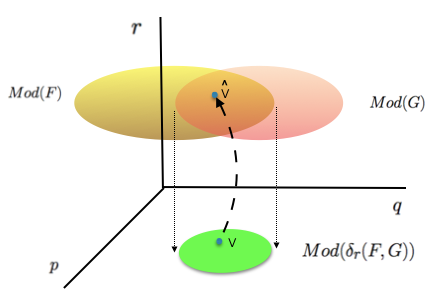
\includegraphics[scale=0.6]{imagenes/indemod.png}
	\caption{Interpretación semántica del operador de omisión (Lema de elevación)}
	\label{fig:proy}
\end{figure}
\vspace{0.5cm}

\lem Sean $v :\mathcal{L} \setminus \{p\} \rightarrow \{ 0,1 \}$ una valoración o interpretación, $F, G \in Form(\mathcal{L})$ fórmulas y $\delta$ un operador de omisión para $p$. Las siguientes condiciones son equivalentes:
\begin{enumerate}
\item $v \vDash \delta (F,G)$
\item Existe una valoración $\hat{v} : \mathcal{L} \rightarrow \{ 0,1 \}$ tal que $\hat{v} \vDash F \wedge G$ y $\hat{v} \upharpoonright_{\mathcal{L} \setminus \{ p \}} = v $
\end{enumerate}

\noindent \textbf{Prueba: } ($1 \Rightarrow 2$): Dada una valoración $v$, se considera la fórmula 
$$H_v = \bigwedge_{q \in \mathcal{L} \{ p \}} q^v$$
donde $q^v$ es $q$ si $v(q)=1$ y $\neg q$ en otro caso. Es claro que $v \vDash H_v$. \\
Supongamos que existe $v \vDash \delta (F,G)$ sin extensiones que modela $F \wedge G$. Entonces la fórmula $H_v \rightarrow \neg (F,G)$ es una tautología, en particular:
$$ \{ F,G \} \vDash H_v \rightarrow \neg (F,G)$$
Como $ \{ F,G \} \vDash F \wedge G$, usando \textit{modus tollens} $\{ F,G \} \vDash \neg H_v$. Así que $\delta (F,G) \vDash \neg H_v$, lo cual es una contradicción porque $v \vDash \delta (F,G) \wedge H_v$
\section{Derivadas Booleanas}

\section{Regla de independencia}

\section{Cálculo lógico}